%\documentclass[10pt,a4paper]{article}
\documentclass[ShortAfour,times,sageapa]{sagej}
\usepackage[utf8]{inputenc}
\usepackage[T1]{fontenc}
\usepackage{amsmath}
\usepackage{amssymb}
\usepackage{graphicx}
\usepackage{longtable}


\begin{document}
	
\runninghead{Luchman}
\title{Relative importance analysis for count regression models}
\author{Joseph N. Luchman\affilnum{1}}
\affiliation{\affilnum{1}Fors Marsh}

\begin{abstract}
	Determining independent variable relative importance is a highly useful practice in organizational science.  Whereas techniques to determine independent variable importance are available for normally distributed and binary dependent variable models, such techniques have not been extended to count dependent variables (CDVs).  The current work extends previous research on binary and multi-category dependent variable relative importance analysis to provide a methodology for conducting relative importance analysis on CDV models using dominance analysis (DA).  Moreover, the current work provides a set of comprehensive data analytic examples that demonstrate how and when to use CDV models in a DA and the advantages general DA statistics offer in interpreting CDV model results.  Moreover, the current work outlines best practices for determining independent variable relative importance for CDVs using replaceable examples on data from the publicly available National Longitudinal Survey of Youth 1979 cohort.  The present work then contributes to the literature by using in-depth data analytic examples to outline best practices in conducting relative importance analysis for CDV models and by highlighting unique information DA results provide about CDV models.
\end{abstract}

\keywords{Dominance Analysis, Relative Importance, Poisson Regression, Negative Binomial Regression, R-square}

\maketitle

\section{Introduction}

	Discrete, infrequent events are common dependent variables in Organizational Science \cite[e.g.,]{bettinazzi2021stakeholder,naumovska2021strength,soda2021networks} and are modeled using \textit{count regression models/CRMs} such as \textit{Poisson regression/PR} or \textit{negative Binomial regression/NBR} \cite{blevins2015count}.   %howto get the 'e.g.,' at the beginning?  use actual examples here?
	
	CRMs differ from the commonly used linear regression model/LRM as their functional forms are exponential or log-linear (i.e., have the form $e^{\sum\beta x}$) to accommodate the necessarily truncated (i.e., non-negative) range of the dependent variable/DV.	
	The log-linear form of CRMs requires the use of new metrics to accurately interpret model results and changes the language that can be used to describe model predictions.
	For example, log-linear CRMs' model coefficients are often interpreted in their exponential form as \emph{incidince rate ratios/IRRs} which describes percentage changes in counts for 1 unit increments to the independent variable/IV.
	In addition, the explained variance $R^2$ does not apply in a straightforward way to log-linear CRMs for describing the quality of model predictions' fit to the data \cite{cameron1996r}.
	
	The way in which count data are constructed also tends to differ from how many continuous, Gaussian distributed variables are constructed that have implications for modeling.
	Count variables are often constructed as aggregated events over a specific time period such as the number of organizations adopting a specific practice in a week \cite{naumovska2021strength} or number of divestitures in a year \cite{bettinazzi2021stakeholder}. 
	For some data, the period of aggregation may differ across observations in the data.
	Such differences might be observed when some observations report outcomes for one year/12 months but some report on outcomes for 9 months.
	These differences in aggregation window can result in different "exposure" to the count generating process and can result in a confound.
	In such circumstances, an additional \emph{offset} variable reflecting the amount of exposure the observation had to the count generating process is introduced to re-establish parity across observations \cite[see, for an example]{glerum2021trainer}.
	In other cases, count data aggregations include observations that "opt out" of the count generating process such as firms choosing not to outsource their patent submissions to a law firm in a year producing 0 patents \cite{somaya2008gone}.
	Such opting out results in \emph{zero inflation}; a situation in which there are more 0 values than would be expected from a Poisson or negative Binomial distribution.  
	Zero inflation can be accommodated by using a specialized zero-inflation model \cite[again see, for an example]{glerum2021trainer}. 
	
	The complexities associated with the use of CRMs as well as those associated with processes used to aggregated count data also extend to considering the use of CRM-based postestimation methods such as relative importance analysis. 
	Relative importance analysis is a widely used model postestimation method that is applied to assist in the interpretation of model results.  
	Specifically, relative importance analysis adds detail to the estimation of parameter estimates and can provide practically useful information about IV predictive utility \cite{tonidandel2011relative}.  
	To date, published methodological work on relative importance analysis has discussed how to apply the method to similarly complex models such as binary \cite{azen2009using}, ordered, and multinomial logit models \cite{luchman2014relative} but has not provided an extensive discussion relative importance analysis with CRMs.
	As was discussed above, there are multiple estimation and data generation complexities with CRMs that are unique and were not discussed in past work on LRM or logit models.
	Thus, extending the literature on relative importance analysis to the unique features of CRMs is an important step toward applying the method to these commonly estimated models in Organizational Science.
	
	The purpose of this work is to provide an extensive discussion of the application of relative importance analysis methods to CRMs.
	First, this manuscript discusses how to use CRMs in \cite[dominance analysis/DA]{azen2003dominance}, a relative importance method with a strong conceptual foundation \cite{gromping2007estimators} and flexible implementation in terms of extensibility \cite[see]{luchman2021determining}.
	A focus of this discussion will be to provide recommendations on the model fit metric to use as well as providing a full data analytic example of how to implement the method with CRMs focusing on PR and NBR.
	Second, this paper provides a detailed discussion of the concepts of exposure and zero inflation with particular attention to issues these two CRM-relevant data generation facets have for computing dominance statistics and determining importance.
	Finally, this paper extends on the work of Blevins, Tsang, and Spain's \cite{blevins2015count} work by discussing how to apply model postestimation methods to assist in adding context and detail to the model results, using their paper's work to choose the correct model given the structure of the data to be analyzed.
	
	In the section below, I begin this work with a detailed discussion of the conceptual background for DA.
	Below I discuss what DA is, why it applies to the results for CRMs, and how it is used to infer the importance of IVs in a predictive model.
		
\section{Dominance Analysis}

	DA is a method that evaluates IV relative importance based on unique contributions to a model fit metric.
	DA is then a methodology that uses empirical results, in particular those related to expected/predicted versus observed differences, to evaluate IV importance.
	The use of predicted versus observed differences is a form of variance-based importance and has a long history in Organizational and Behavioral Science as a method for inferring importance \cite[see]{johnson2004history}.
	What makes DA unique among variance-based importance methods is DA's conceptual foundation as an extension of Shapley value decomposition from Cooperative Game Theory % needs caps?
	\cite{}.
	
	\subsection{Shapley Value Decomposition}
	
	Cooperative games can be thought of as a structured form of interaction in which the interacting parties are required to work together toward a common goal and share information with one another (cite).
	This form of interaction is not unlike a team task where the different team members have different pieces of information or different tools and must cooperate to accomplish the task.
	The Shapley value decomposition methodology then uses the structure of the game to determine the unique value ascribed to each player independent of other players irrespective of potentially overlapping player contributions.
	Computationally, the Shapley value computation is the average increment to the obtained cooperative value a player obtains across all possible permutations of coalitions. 
	Formally, player A's ($Pl_a$) Shapley value would be:
	
	\begin{equation}
		SV_{Pl_a} = \frac{\sum_{i=1}^{P} V_{O_i \cup Pl_a} - V_{O_i}}{P}
	\end{equation}

	Where $P$ refers to the total number of permutations of the $p$ players and $O_i$ is some distinct ordered set (i.e., where the order of inclusion matters) of players not including $Pl_a$ that can include the null set of no players.
	
	Predictive models work in a way similar to cooperative games in that IVs jointly enter into a predictive equation (i.e., must interact) and are adjusted for redundancy in terms of prediction of the DV (i.e., share information).
	Thus, Shapley value decomposition can be applied in a straightforward way to predictive models if the IVs are thought of as players and the fit statistic is thought of as the cooperative goal value.
	Indeed, the Shapley value methodology has received a great deal of attention recently in the machine learning literature as a general, model agnostic method for understanding complex model predictions \cite[e.g., ]{lundberg2020local}.
	Moreover, the generality of the Shapley value decomposition methodology means that the approach extends in a natural way to the decomposition of CRM values. 
	Shapley values are a general method for decomposing values but its extension to DA is the methodology that most clearly defined methods for determining the relative importance of predictive models.
	
	\subsection{General Dominance Statistics}
	
	The \emph{General Dominance Statistic} in the DA approach to relative importance is directly related to the Shapley value computation but is focused on decomposing a model fit metric and simplifies the Shapley value computation given the features of fit metrics.
	The simplification general dominance statistics apply is based on the acknowledgment that, for a predictive model, the ordering of IV input is usually irrelevant.  That is, the order of inclusion for fit metrics in predictive models tends to produce equal fit statistics (i.e, $R^{2}_{IV_{x}IV_{z}} = R^{2}_{IV_{z}IV_{x}}$).	
	Computationally, the general dominance statistic for an IV ($IV_x$) is:
	
	\begin{equation}
		GDS_{IV_x} = \sum_{j=1}^{TCb} \frac{ F_{U_j \cup IV_x} - F_{U_j}}{(C_{U_j \cup IV_x}) k}
	\end{equation}
	
	Where $TCb$ refers to the total number of unique combinations not including $IV_x$ (i.e., $2^{k-1}$) of the $k$ IVs, $U_j$ is some distinct unordered set (i.e., where the order of inclusion doesn't matter) of IVs not including $IV_x$ that can include the null set of no IVs, and $C_{U_j \cup IV_x}$ is the number of distinct combinations of IVs with all the IVs in $U_j$ as well as $IV_x$ included in the model.		
	The general dominance statistics are then generated as a weighted-average increment to the fit metric across all combinations of IVs to which the focal IV is included.
	The weighted averaging component of the denominator of Equation 2 reflects the idea that there are redundancies in the Shapley value computation that can be rescaled such that they can be reflected by a weighted average.
	
	The general dominance statistics are used to determine importance among the IVs by comparing their values.
	For example, if $IV_x$ has a larger general dominance statistic than $IV_z$, $IV_x$ is said to \emph{generally dominate}, and is thus more important than, $IV_z$.
	
	DA extends on Shapley value composition further in the next section that discusses two other importance designations used in DA to make stronger importance determinations than that which general dominance statistics are capable.
	
	\subsection{Other Dominance Computations and Designations}
	
	DA also computes statistics known as a \emph{conditional dominance statistic} that is closely related to the general dominance statistic.  
	The conditional differs from the general dominance statistic as it is computed by a specified number of IVs included in the model.
	Thus, each IV has $k$ conditional dominance statistics.
	The conditional dominance statistic for an IV ($IV_x$) with a set number of IVs in the model ($s$) is computed:
	
	\begin{equation}
		CDS_{IV_x}^{s} = \sum_{l=1}^{C_{U_l \cup IV_x}} \frac{ F_{U_l \cup IV_x} - F_{U_l}}{C_{U_l \cup IV_x}}
	\end{equation}

	Where $U_l$ is some distinct unordered set of $s-1$ IVs not including $IV_x$ that can include the null set of no IVs, and $C_{U_l \cup IV_x}$ is the number of distinct combinations of the $s$ IVs with all the IVs in $U_l$ as well as $IV_x$ included in the model.
	
	Conditional dominance statistics computed using Equation 3 are a subset of the computations in the general dominance statistic in Equation 2 and can be averaged to obtain the general dominance statistic.  
	That is, $GDS_{IV_x} = \sum_{g=1}^{k} \frac{CDS_{IV_x}^{g}}{k}$.
	
	The conditional dominance statistics generated for each IV are also used to determine importance among the IVs but the procedure for doing so requires a different approach than that applied to general dominance statistics.
	For conditional dominance statistics, if, within a number of IVs in the model, all of $IV_x$'s values are larger than $IV_z$, $IV_x$ is said to \emph{conditionally dominate}, and is thus more important than, $IV_z$.
	Another way of thinking about conditional dominance is that, if the conditional dominance statistics for an IV were graphed as a line by the number of IVs in the model, $IV_x$'s value is above $IV_z$ value for the entirety of the trend.	
	Because conditional dominance statistics are a 'less averaged' version of the general dominance statistics, conditional dominance of one IV over another is a stricter criterion than general dominance and implies a stronger form of IV relative importance.
	
	DA also uses a third type of comparison called \emph{complete dominance} that does no averaging at all.
	In complete dominance, each increment to the fit metric associated with $IV_x$ is compared to an corresponding increment for $IV_z$.
	More formally, for all sets of IVs $U_q$ that do not include $IV_x$ or $IV_z$ and can include the null set of no IVs, $F_{U_q \cup IV_x} - F_{U_q}$ is always larger than $F_{U_q \cup IV_z} - F_{U_z}$.
	In such situations, $IV_x$ is said to \emph{completely dominate} $IV_z$.
	Because there is no averaging involved in the comparisons that produce complete dominance, it is the most stringent importance comparison between two IVs.
	
	This section has outlined why Shapley value decomposition and the extension into DA applies to CRMs. 
	This section has also provided a discussion of how DA statistics and designations are computed and determined.
	In the section below, I transition from a broad outline of DA to a more targeted discussion of the application of DA to CRMs.
	The discussion of CRM-based DA begins by considering which fit metric should be used and proceeds to an extensive example applying DA to both PR and NBR.
	
\section{Applying Dominance Analysis to Count Regression Models}

	Conceptually, DA can be applied to CRMs as its basis in Shapley values allows the application of the method to any procedure that is similar to a cooperative game.
	A complication of applying DA to CRMs is that most of the literature on DA has focused on its application to LRM with the residual $R^2$ (i.e., $R^2_{RES}$).
	CRMs and LRM have many similarities and, given the numerical nature of count DVs and that the output from CRMs is typically in the form of a predicted count/mean value, the $R^2_{RES}$ could be applied to CRM-based DA.
	
	Although $R^2_{RES}$ could be applied, there are good conceptual reasons to choose another fit metric. 
	The section below provides a detailed rationale for the choice of a different metric, the deviance $R^2$ (i.e., $R^2_{DEV}$), that better reflects how CRMs fit to data. 
	
	\subsection{Count Regression Fit Metric: Deviance $R^2$}
	
	CRMs are not only log-linear models but also follow probability distributions that differ from the LRM that has been traditionally been the focus of DA.
	This is important as statistical models are fit using information about the data as applied to a probability distribution to find their most likely parameter values.
	It is thus important to choose a fit metric that matches the probability distribution's underlying fitting criterion.
	
	First consider LRM.
	LRM is based on a Normal or Gaussian probability distribution that can be simplified to the	least-squares criterion which seeks to minimize $\sum (y - \hat{y})^2$ or the sums of squares between the predicted values from the LRM and the observed DV.
	The $R^2_{RES}$ that has been traditionally applied in LRM-based DA is one less than the ratio of the sum of squares of the observed DV and predicted value to the sum of squares of the observed DV and the mean of the observed DV (i.e., $\sum (y - \bar{y})^2$).
	Because the $R^2_{RES}$ uses the LRM minimization goal's in computing differences between the observed data and the predictions, the $R^2_{RES}$ is a useful model fit metric for LRM.
	
	The $(y - \hat{y})^2$ computation used in the computation of the $R^2_{RES}$ is also known as the \emph{unit deviance} for the Normal distribution as it describes how the model's prediction "deviates" from observed values \cite{mccullagh2019generalized}.
	The value in the numerator of the $R^2_{RES}$ is then a deviance for a Normal distribution.
	The denominator can be similarly cast as a deviance if considering a null LRM that estimates only an intercept and thus returns the mean.
	Thus, the the $R^2_{RES}$ can also be thought of as a deviance $R^2$.
	
	Cameron and Windmeijer \cite{cameron1996r} first formalize the concept of extending the $R^2_{RES}$ to a version of the metric based on deviance.
	The deviance $R^2$ is computed as:
	
	\begin{equation}
		R^{2}_{DEV} = 1 - \frac{D_{model}}{D_{null}}
	\end{equation}

	Where $D_{null}$ is the model deviance associated with a null model describing an intercept- or mean-only model.
	Thus, when the LRM's deviance computations are substituted in for the $D_{model}$ and $D_{null}$ values, the $R^{2}_{DEV}$ is equivalent to $R^{2}_{RES}$.
	
	An advantage of constructing the $R^{2}_{DEV}$ is that the deviance concept has been generalized from LRM to generalized linear models such as PR and NBR as well.
	For example, the unit deviance computation for PR and a special case of the NBR\footnote{This special case is the NBR estimated using a quasi-likelihood method. Maximum likelihood methods require a more complex form given the estimation of the $\alpha$ parameter.} is $2(y\ln \frac{y}{\hat{y}} - (y - \hat{y}))$. 
	This PR-focused deviance value differs notably from the Normal distribution deviance in that it tends to penalize underprediction more than overprediction.
	The extra penalties assigned to underprediction are consistent with the PR's log-linear nature in that the log distance between 1 and 2 (.69) is larger than between 2 and 3 (.41); on average, lower log-transformed differences get penalized more than higher log-transformed differences.
	By contrast, Normal distribution deviance penalizes discrepancies from observed values equally in either direction.
	
	The $R^{2}_{DEV}$ is then a useful generalization of the $R^{2}_{RES}$ that allows the researcher to apply an residual computation that makes sense for the model in question, as opposed to applying the LRM's deviance criterion to a model that is not based on LRM \cite[.e.g.,]{cameron1996r}.
	The $R^{2}_{DEV}$ is then the fit metric recommended for use in conducting DA with CRMs.
	
	This section has provided a rationale for the choice of a specific fit metric to use when applying DA to CRMs.
	In the sections to follow, I transition to the description of the methodology for applying DA to CRMs.
	This discussion briefly outlines the data generated for this purpose, describes the models estimated from the data, and also describes how DA statistics and designations were determined with the results.
	
	\subsection{Count Regression Model-based Dominance Analysis: An Analytic Example}
	
	In this section I describe how I generated data for a both a PR and NBR model.
	These models are estimated in such a way as they would be were they based on "real" data and follow a procedure similar to that that would be applied to answering a "real" research question with the data.
	
	The next section provides a high-level overview of how the data were generated and descriptive statistics about the data.
	Note that a full outline of the data generation and analysis process is available in the online supplement.
	
		\subsubsection{Data Generation}
		
	The data for this analysis were generated as opposed to obtained empirically to maintain control over their usefulness in illustrating the key concepts for this manuscript.
	A goal in generating these data were to make them "realistic" when possible. 
	That is, to reduce the elements of the data that made them simulated in order to focus on the concepts
	
	The data simulated in this section were intended to describe the generation of garments from a tailors in a fortnight or two-week period.
	Data from a total of 6,780 simulated tailors were generated over this period across two different garments/DVs and for four garment generation factors/IVs.
	
	One dependent variable, the number of stock sport coats of a set size made by the tailors, is Poisson distributed. 
	The second dependent variable, number of made-to-measure sport coats with custom elements made by the tailors, is negative Binomial distributed. 
	The four garment generation factors include a] equipment reliability, b] assistant staffing levels, c] tailor skill-level, and d] tailor work experience.
	Each of the four garment generation factors were designed to be multivariate Normally distributed with pre-specified relationships with the two forms of garment count DVs.
	The pre-specified relationships between each of the garment generation factors with both garment count DVs were identical.
	The only factor that differed between garment generation factors was the distribution of the DV.
	Both garment count DVs were designed to have mean values of 1.
	The negative Binomial, made-to-order sport coat count variable was also designed to have a variance of 3.	
	
	The means, standard deviations, and correlations between all four IVs and two DVs is reported below in Table 1. 
	
\begin{longtable}{lrr|rrrrrr}
	\caption*{
		{\large Table 1: Descriptive Statistics}
	} \\ 
	\toprule
	&  & Standard & \multicolumn{6}{c}{Correlations} \\ 
	\cmidrule(lr){4-9}
	Variable & Mean & Deviation & ER & AS & SL & WE & SJ & MJ \\ 
	\midrule
	ER & $-0.0355$ & $1.1853$ & $1.0000$ & $0.4168$ & $0.1446$ & $0.2180$ & $0.3734$ & $0.3237$ \\ 
	AS & $-0.0261$ & $1.4494$ & $0.4168$ & $1.0000$ & $0.1958$ & $0.2850$ & $0.3954$ & $0.3425$ \\ 
	SL & $-0.0056$ & $1.5480$ & $0.1446$ & $0.1958$ & $1.0000$ & $0.3295$ & $0.3410$ & $0.2967$ \\ 
	WE & $0.0144$ & $1.9211$ & $0.2180$ & $0.2850$ & $0.3295$ & $1.0000$ & $0.3586$ & $0.3188$ \\ 
	SJ & $0.9963$ & $1.0090$ & $0.3734$ & $0.3954$ & $0.3410$ & $0.3586$ & $1.0000$ & $0.8773$ \\ 
	MJ & $1.0000$ & $1.7571$ & $0.3237$ & $0.3425$ & $0.2967$ & $0.3188$ & $0.8773$ & $1.0000$ \\ 
	\bottomrule
\end{longtable}

	Table 1 shows that the means of each of the IVs are 0 and the means of the DVs are 1. 
	Table 1 also shows variability between the IVs in terms of their variances with ER having the lowest variability and WE the highest.
	The results also show modest to moderate-sized correlations between IVs with SL having some of the lowest overlap with other IVs and AS having the highest.
	The results for the DVs also show distinctly different standard deviations with SJ following the Poisson distribution requirement that the mean equal the variance and MJ showing a much higher variation than the mean as is typical of negative Binomial distributed variables.
	
	The next section moves on to using these data to estimate a PR with the SJ variable as well as an NBR with the MJ variable predicted by the four IVs.

		\subsubsection{Regression Results}
		
	The PR results predicting SJ are reported in Table 2. 
	
	\begin{longtable}{l|rrrrrrrr}
		\caption*{
			{\large Table 2: Poisson Regression}
		} \\ 
		\toprule
		\multicolumn{1}{l}{} &  &  & \multicolumn{2}{c}{Confidence Interval} &  &  &  &  \\ 
		\cmidrule(lr){4-5}
		\multicolumn{1}{l}{} & Coefficient & SE & Low & High & z & p & IRR & Standardized \\ 
		\midrule
	\(Intercept\) & $-0.1509$ & $0.0139$ & $-0.1782$ & $-0.1239$ & $-10.8831$ & $0.0000$ & $0.8599$ & $0.0000$ \\ 
		ER & $0.1817$ & $0.0114$ & $0.1593$ & $0.2040$ & $15.9313$ & $0.0000$ & $1.1992$ & $0.2154$ \\ 
		AS & $0.1532$ & $0.0095$ & $0.1346$ & $0.1718$ & $16.1525$ & $0.0000$ & $1.1655$ & $0.2220$ \\ 
		SL & $0.1381$ & $0.0083$ & $0.1218$ & $0.1544$ & $16.5715$ & $0.0000$ & $1.1481$ & $0.2138$ \\ 
		WE & $0.0981$ & $0.0069$ & $0.0846$ & $0.1116$ & $14.2399$ & $0.0000$ & $1.1031$ & $0.1884$ \\ 
		\bottomrule
	\end{longtable}

	Table 2 shows that ER had the largest unstandardized coefficient and IRR value with a 1 unit change in equipment reliability leading to a 19.9\% increase in the number of stock jackets produced in a fortnight.
	By contrast, WE obtained the smallest unstandardized coefficient and IRR value with a 1 unit change in equipment reliability leading to a 10.3\% increase in the number of stock jackets produced in a fortnight. 
	AS and SL fell between ER and WE in terms of unstandardized coefficient/IRR results.
	
	The standardized coefficients, computed on each of the IVs standardized to have a variance of 1, show a different ordering of the IVS. 
	In contrast to the unstandardized results, the biggest coefficient for the standardized results was associated with AS with ER a close second. 
	Hence, the magnitude of the unstandardized coefficients was scale dependent.
	This scale dependence is a well-known drawback of the use of use of unstandardized coefficients for comparing effects across IVs.
	
	The NBR results predicting MJ are reported below in Table 3.
	
\setlength{\LTpost}{1mm}
\begin{longtable}{l|rrrrrrrr}
	\caption*{
		{\large Table 3: Negative Binomial Regression}
	} \\ 
	\toprule
	\multicolumn{1}{l}{} &  &  & \multicolumn{2}{c}{Confidence Interval} &  &  &  &  \\ 
	\cmidrule(lr){4-5}
	\multicolumn{1}{l}{} & Coefficient & SE & Low & High & z & p & IRR & Standardized \\ 
	\midrule
	\(Intercept\) & $-0.3936$ & $0.0207$ & $-0.4341$ & $-0.3533$ & $-19.0401$ & $0.0000$ & $0.6747$ & $0.0000$ \\ 
	ER & $0.3026$ & $0.0174$ & $0.2683$ & $0.3370$ & $17.4069$ & $0.0000$ & $1.3533$ & $0.3586$ \\ 
	AS & $0.2589$ & $0.0144$ & $0.2305$ & $0.2874$ & $17.9264$ & $0.0000$ & $1.2955$ & $0.3752$ \\ 
	SL & $0.2361$ & $0.0127$ & $0.2111$ & $0.2613$ & $18.5623$ & $0.0000$ & $1.2663$ & $0.3656$ \\ 
	WE & $0.1702$ & $0.0105$ & $0.1497$ & $0.1909$ & $16.1851$ & $0.0000$ & $1.1856$ & $0.3270$ \\ 
	\bottomrule
\end{longtable}
\begin{minipage}{\linewidth}
	Theta parameter is 1.116105.\\
\end{minipage}

	Table 3's unstandardized/IRR results are similar to those of Table 2 in terms of ranking of magnitudes but produced larger values.
	ER remained the largest IRR in the NBR with a 1 unit change in equipment reliability leading to a 35.3\% increase in the number of stock jackets produced in a fortnight.
	WE remained the smallest IRR in the NBR with a 1 unit change in equipment reliability leading to a 18.6\% increase in the number of stock jackets produced in a fortnight.
	
	...ended here ...
	
	
	Table X3 shows that the most substantial slope size obtained by any of the IVs is for $IV_4$ with a value of .294.  
	A one unit change in $IV_4$ then produces a 0.294 change in $Y_{Normal}$.
	Compare $IV_4$'s results with those obtained from $IV_2$.
	$IV_2$ obtained the smallest value for its coefficient with 0.049.
	A one unit change in $IV_2$ then produces a 0.049 change in $Y_{Normal}$.	
	The combination of four coefficients presented in Table X3 resulted in an explained variance $R^2$ of .1125.
	
	
	The values obtained by the IVs in Table X3 were, effectively, the population values reported on earlier in the manuscript. 
	This result occurred as the LRM is correctly specified and, as such, the correct, known parameter estimates for each of the IVs is recovered.
	Thus, as noted above, the potentially surprising results observed of the IV-DV correlations is an artifact of the IV interrelationships and does not carry over to the parameter estimates.
	
	The coefficients in Table X3 are unstandardized which makes their interpretation comparable only when their variances are equal.
	This is because one unit changes in IVs differ in their 'typical'-ness and how well they reflect change in an IV.
	For instance, the standard deviation of $IV_4$ (1.15) is closest to a value of 1 of all the IVs.  
	The unstandardized coefficient for this IV then describes this variable's effect best in terms of typical changes.
	By contrast, $IV_1$ has a standard deviation of 0.30.
	Thus, a 1 unit change is far from typical and actually describes a nearly 3 standard deviation change in that IV.
	The comparisons between the coefficients can be improved by standardization where the typical changes are harmonized such that they all reflect one standard deviation of change.
	When standardized, the results from the LRM show slightly different trends.
	$IV_4$ remains strongest with a standardized coefficient of 0.338.
	For every one standard deviation change in $IV_4$ there is a 0.338 standard deviation change in $Y_{Normal}$.  
	The standardized value for $IV_4$ remained similar to it's value when unstandardized as its variance was near 1.
	Note however the substantial change to $IV_1$ which had an unstandardized value very close to $IV_4$'s value but a standardized value (0.080) that is around 30\% of its unstandardized value.
	This is because, as noted above, the typical change for $IV_1$ is around 0.30; 30\% of the value of 1 assumed with an unstandardized coefficient.
	
	The standardized as compared to the unstandardized results in Table X3 show that there are interpretive challenges for this model given the differing variances and coefficient values and attempting to determine which IVs are most important.  
	The results in Table 3 will be revisited below when considering the DA results for the LRM. 
	The CRM results predicting $Y_{Poisson}$ are presented next.
	
	The CRM results for $Y_{Poisson}$ are reported in Table X4.
	
	\begin{longtable}{l|rrrrrrr}
		\toprule
		\multicolumn{1}{l}{} & Coefficient & SE & z & p & CI\_low & CI\_high & Std\_Coefficient \\ 
		\midrule
		\(Intercept\) & $-0.049$ & $0.003$ & $-14.889$ & $0.000$ & $-0.056$ & $-0.043$ & $0.000$ \\ 
		IV1 & $0.237$ & $0.012$ & $19.994$ & $0.000$ & $0.213$ & $0.260$ & $0.072$ \\ 
		IV2 & $0.046$ & $0.009$ & $5.141$ & $0.000$ & $0.029$ & $0.064$ & $0.025$ \\ 
		IV3 & $0.107$ & $0.004$ & $25.926$ & $0.000$ & $0.099$ & $0.115$ & $0.091$ \\ 
		IV4 & $0.269$ & $0.004$ & $70.957$ & $0.000$ & $0.262$ & $0.277$ & $0.308$ \\ 
		\bottomrule
	\end{longtable}
	
	Table X4, like the results from X3, shows that the most substantial slope size obtained by any of the IVs is for $IV_4$ with a value of 0.269.
	By comparison with the LRM results, the PR results are not as readily interpretable in their linearized form as it indicates that a one unit change in $IV_4$ then produces a 0.269 change in the natural logarithm of $Y_{Poisson}$.
	A more useful way to interpret $IV_4$'s result is in IRR/exponentated form as $e^{.269} \approx 1.309$.
	The IRR for $IV_4$ then indicates that a one unit change in $IV_4$ results in a 30.9\% increase in the value of $Y_{Poisson}$.
	As is discussed above, CRMs are multiplicative models and their results increase in percentages as opposed to strictly additively like the LRM.
	Again, $IV_2$ obtained the smallest value for its coefficient with 0.046 or an IRR of $e^{0.046} \approx 1.047$.
	A one unit change in $IV_2$ then produces a 4.7\% increase in $Y_{Poisson}$.
	The combination of four IVs in Table X4 produced a $R^2_{DEV}$ of .0814.
	
	The CRM results suffer, like the LRM results, from interpretive challenges due to the variances of the IVs and can be similarly standardized\footnote{Standardized coefficients for the Poisson model were generated by standardizing the IVs and ...}.
	The standardized CRM results remain multiplicative but are interpreted in standard deviation change terms.
	$IV_4$'s value of 0.308 can be interpreted as a one standard deviation change in $IV_4$ is associated with a $e^{0.308} \approx 1.361$ or 36.1\% increase in $Y_{Poisson}$.
	
	Before moving on, as the reader has no doubt observed, $Y_{Poisson}$'s CRM results are, as intended, numerically similar to those obtained from the results for $Y_{Normal}$ LRM.
	Again, these results were intended to show the strong similarities across models in many aspects that, as I intend to show, carry over to the determination of importance using DA.
	The most noteworthy difference between the CRM and LRMs is the non-zero intercept value for the PR model which reflect the baseline incidence rate of $e^{-0.049} \approx 0.952$. 
	Because the baseline incidence rate is the incidence rate when each of the IVs is 0, it reflects the value at the means of each of the IVs; the value of nearly 1 indicates that the known mean of $Y_{Poisson}$ is achieved, as expected, when all IVs are at their means.	
	
	The LRM and CRM's unstandardized and standardized coefficients have been discussed at length in the preceeding section.
	The next section transitions to discussing how the DA process is implemented with both the LRM and CRM and interpreting their DA statistics.
	
		\subsubsection{Dominance Analysis Results}
		
	The DA results for both the LRM and CRM are based on the series of $R^2$ values each associated with different subsets of IVs reported in Table X5.
	
	\begin{longtable}{lrr}
		\toprule
		formula & \$R\textasciicircum{}2\_\{Y\_\{Normal\}\}\$ & \$R\textasciicircum{}2\_\{Y\_\{Poisson\}\}\$ \\ 
		\midrule
		Y \textasciitilde{} IV1 & $0.0061$ & $0.0044$ \\ 
		Y \textasciitilde{} IV2 & $0.0284$ & $0.0205$ \\ 
		Y \textasciitilde{} IV1 + IV2 & $0.0521$ & $0.0375$ \\ 
		Y \textasciitilde{} IV3 & $0.0023$ & $0.0017$ \\ 
		Y \textasciitilde{} IV1 + IV3 & $0.0096$ & $0.0070$ \\ 
		Y \textasciitilde{} IV2 + IV3 & $0.0284$ & $0.0205$ \\ 
		Y \textasciitilde{} IV1 + IV2 + IV3 & $0.0521$ & $0.0375$ \\ 
		Y \textasciitilde{} IV4 & $0.0984$ & $0.0711$ \\ 
		Y \textasciitilde{} IV1 + IV4 & $0.1042$ & $0.0753$ \\ 
		Y \textasciitilde{} IV2 + IV4 & $0.0988$ & $0.0714$ \\ 
		Y \textasciitilde{} IV1 + IV2 + IV4 & $0.1046$ & $0.0756$ \\ 
		Y \textasciitilde{} IV3 + IV4 & $0.1045$ & $0.0757$ \\ 
		Y \textasciitilde{} IV1 + IV3 + IV4 & $0.1122$ & $0.0812$ \\ 
		Y \textasciitilde{} IV2 + IV3 + IV4 & $0.1076$ & $0.0780$ \\ 
		Y \textasciitilde{} IV1 + IV2 + IV3 + IV4 & $0.1125$ & $0.0814$ \\ 
		\bottomrule
	\end{longtable}

	The $R^2$ values associated with each model are reported together in this section to, again, highlight the similarities across models in terms of how the IVs explain variability or reduce deviance in the DV.
	The final value for the LRM and CRM were reported above and reflect the value of the $R^2$ to be decomposed by the DA procedure for importance determination.
	
	The results in Table X5, when applied to Equation 3?, produce the General Dominance Statistics for the LRM and CRM reported on in Table X6.
	
	\begin{longtable}{l|rrr}
		\toprule
		\multicolumn{1}{l}{} & General\_Dominance & Percent & Ranks \\ 
		\midrule
		\multicolumn{4}{l}{Normal} \\ 
		\midrule
		IV1 & $0.0089$ & $0.0793$ & 3 \\ 
		IV2 & $0.0171$ & $0.1515$ & 2 \\ 
		IV3 & $0.0048$ & $0.0424$ & 4 \\ 
		IV4 & $0.0818$ & $0.7268$ & 1 \\ 
		\midrule
		\multicolumn{4}{l}{Poisson} \\ 
		\midrule
		IV1 & $0.0064$ & $0.0785$ & 3 \\ 
		IV2 & $0.0123$ & $0.1509$ & 2 \\ 
		IV3 & $0.0035$ & $0.0435$ & 4 \\ 
		IV4 & $0.0592$ & $0.7270$ & 1 \\ 
		\bottomrule
	\end{longtable}

	There are a series of points of note from the results presented in Table X6.
	First, $IV_4$ generally dominated all three other IVs and by a wide margin for both the LRM and CRM results.
	Moreover, $IV_4$ has been ascribed nearly 73\% of all the explained variance/reduced deviance across both models.
	This result is not surprising given $IV_4$'s coefficient results and variance which show both a high amount of variability coupled with a large regression coefficient.
	
	Second, one perhaps surprising result is that $IV_2$, the IV with the smallest coefficient and second smallest variance, obtained the second largest general dominance statistic, generally dominating both $IV_1$ and $IV_3$.
	This result is related directly to the pattern of intercorrelations observed in Table X1.
	$IV_2$ has the second largest correlation with the DVs and the strongest observed correlations with the other IVs.  
	As a result of $IV_2$'s overlap with other IVs, it is more difficult to distinguish how much explained variability in each DV \emph{should} be ascribed to $IV_2$.
	In fact, the strong correlation $IV_2$ has with other IVs allows it to 'borrow' other IVs' predictive usefulness as it is unclear how to parse the predicted values produced by $IV_2$ relative to other IVs as they appear to correspond so strongly in the data.
	The Shapley Value decomposition method underlying DA tends to split the difference between IVs when it is unclear as to how to subdivide fit statistic's value.
	It is worth noting that the next set of results, focusing on the conditional dominance statistics, are insightful for showing how $IV_2$ resulted in being second most important across subsets of models.
	
	Finally, as has been implied in the discussion of the general dominance results, the LRM and CRM based general dominance statistics are similar; in fact the Percentage of the $R^2$ values explained by each IV are identical to two decimal places.
	The general dominance statistic results then support my contention that CRM-based DA is a straightforward extension of LRM-based DA using an $R^2$ that is computed slightly differently but is conceptually identical to the explained variance $R^2$.
	
	The next section discusses the more conditional dominance statistics; which as sub-components of the general dominance statistics.
	
	The results for the LRM and CRM-based DA conditional dominance statistics are reported in Figure X1. 
	The graphic format is useful with conditional dominance statistics as it makes the trends across number of IVs included in the model, as well as conditional dominance determination, easier to see.
	 
	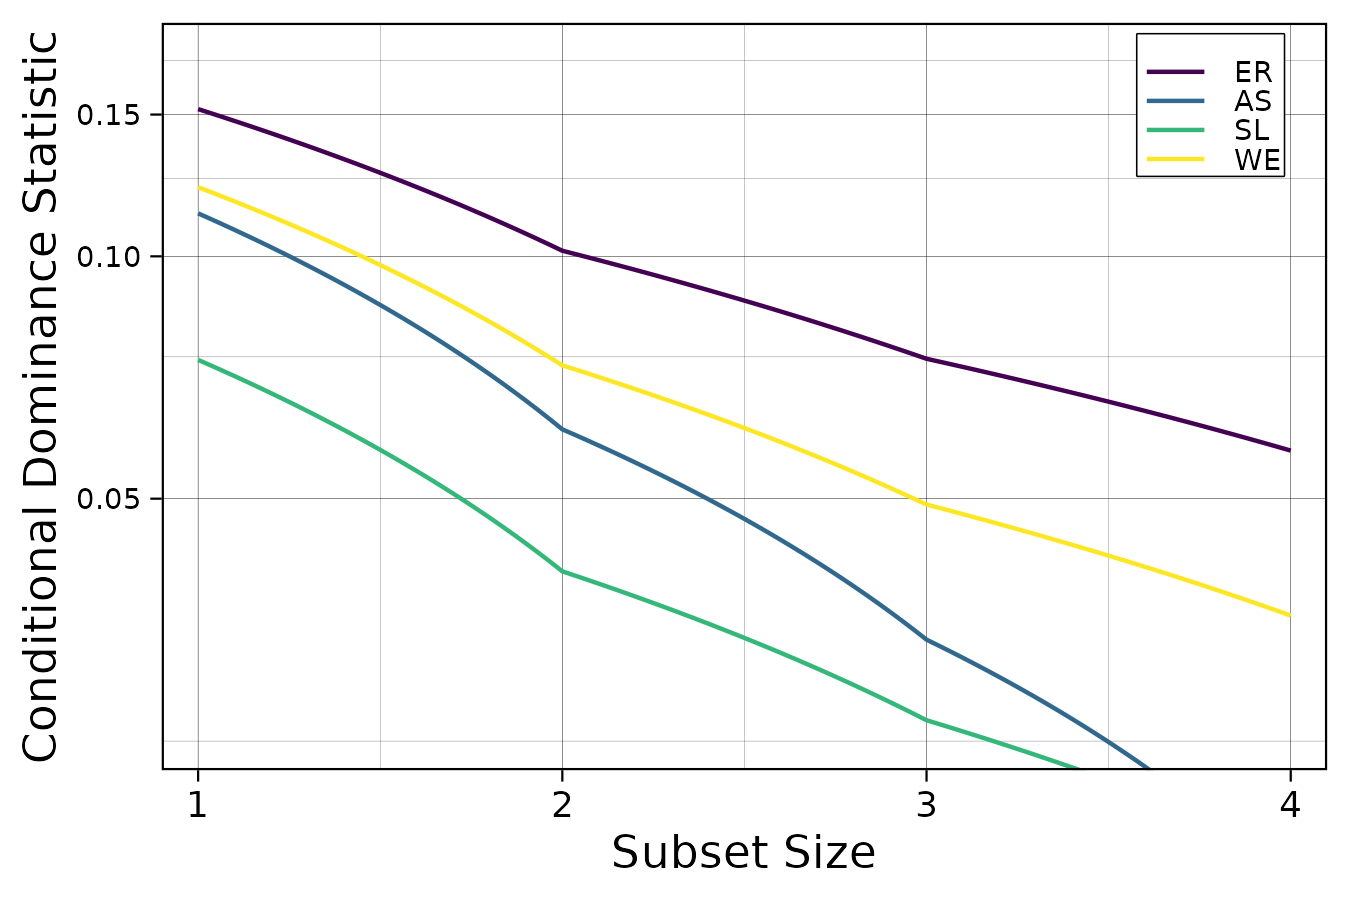
\includegraphics{includes/condit_gph}
	
	Figure X1 shows that $IV_4$ conditionally dominates all three of the other IVs.
	By contrast, the three other IVs have no conditional dominance relationships.
	This is because the three lines describing $IV_1$, $IV_2$, and $IV_3$'s conditional dominance statistics cross over one another between the three IV and all 4 IV in the model.
	
	It is worth noting that the ordering of the conditional dominance statistics at 4 IVs in the model for the LRM and CRM mirror the order of the standardized coefficient magnitudes ... whereas for 3 IVs or less in the model the ordering match the order of the correlations with the DV...
	
	The conditional dominance statistics reinforce the similarity across LRM and CRM DA results as the trends for each IV across numbers of IVs in the model are nearly identical.
	Again, the difference between LRM-based DA and CRM-based DA is primarily in the choice of fit metric and underlying predictive model; implementation between both is identical and, when the results are designed to be similar, the DA statistics produced are similar.
	
	The $R^2$ values in Table X5 can also be used to determine complete dominance of IVs over one another.  
	Because $IV_1$, $IV_2$, and $IV_3$ have no conditional dominance designations over one another, they cannot have complete dominance designations.
	$IV_4$ does conditionally dominate each of $IV_1$, $IV_2$, and $IV_3$; thus, $IV_4$ could possible also completely dominate each other IV.  
	The pattern of $R^2$ values in Table X5 shows that for both the LRM and CRM results, $IV_4$ completely dominates $IV_1$, $IV_2$, and $IV_3$.
	
	\subsubsection{Section Summary}
	
	This section intended to provide a detailed example of the estimation of both a LRM and CRM as well as DAs based on those models.
	The examples provided were based on generated data that were produced with the intention of being (reasonably) realistic as well as being as comparable as possible across LRM and CRM results.
	The data analytic examples of DA presented provide empirical evidence for the theoretical expectation that a LRM and CRM that are based on the same underlying causal structure should produce similar DA results.
	This demonstration thus serves to illustrate the straightforward generalization of DA from LRM to CRMs.
	
	Although DA with both LRM and CRMs can produce similar results when sharing an underlying causal structure, there are additional complexities to CRM estimation that do not have similar analogs with LRM given the data generating mechanisms underlying count DVs.
	The discussion of DA with CRMs turns, in next section, to a more extensive discussion of this additional complexity and when it can impact DA statistics and determinations.
	
	
	%this part below (other than final transition) needed in this section?
	The data for the analytic examples were generated using R \cite{R} using a combination of base R's \texttt{stats} package as well as the \texttt{MASS} package \cite{MASS}.  
	Other details of data generation for the reproducibility of the analysis can be found in Appendix X.  
	The section below transitions from discussing data generation processes to data analysis.
%	
%	\subsection{Base Relative Importance Results}
%	
%	The data generated above by data structure and DV distribution were submitted to separate DAs to produce a total of twelve different DAs.
%	The four DAs with each Normally distributed DV was based on linear regression.
%	The four DAs with each Poisson distributed DV was based on Poisson regression/generalized linear model with a log link and Poisson family.
%	The four DAs with each negative Binomial distributed DV was based on negative Binomial regression/generalized linear model with a log link and negative Binomial family.
%	The model parameter estimates for each of the twelve models DAs were also estimated but are not reported in this section as they are not a focus; these results are reported in Appendix X. 
%	The general dominance statistic results from each DA are presented in table X.
%	
%	
%		\subsubsection{Linear Model}
%	
%	The results from the linear model-based DA is, as noted above, most useful in this table as a comparison point for the other results computed from the CRMs.
%	The linear model is used as a comparison point as it is a better known model than most CRMs and is easier to work with mathematically.
%	The EU data structure is also intended to be a comparison point data structure representing idealized, if unrealistic, data conditions for estimation.
%	As such, I begin the interpretation of the results with the EU data.	
%	The idealized data structure represented by the EU condition produced results that were consistent with those which would be theoretically expected with identically distributed, uncorrelated IVs.  
%	Specifically, when there are no intercorrelations and the variance of the variable is 1, the expected $R^2$ value is the square of the coefficient (cite?).
%	The linear model results in Table X for the EU data structure follow this pattern well and show that general dominance statistic results, when there are no intercorrelations and equal variances, recover the theoretically expected $R^2$ values.  
%	Indeed, as is well known (cite?), DA is not a necessary procedure when IVs are not intercorrelated as the incremental $R^2$ values for each IV are tantamount to the general dominance statistics.
%	
%	% report the conditional dominance and complete stats too?
%	
%	The UU results vary from those obtained by the EU in that $V_4$, despite having a known coefficient value that is half that of $V_1$ obtained nearly the same general dominance statistic value.
%	As with the EU structure, UU's results are theoretically known.
%	For variables with unequal variances with no intercorrelations, the expected $R^2$ value is the square of the coefficient times the IV variance (cite?).
%	Hence, the expected general dominance statistics for $V_1$ and $V_4$ in the UU data structure were theoretically the same (i.e., $C_{V_1} = .2^2*1 = .1^2*4 = C_{V_4}$) however as realized in data as simulated in this manuscript, $V_1$ gained a slight edge and generally dominates $V_4$.
%	The results from the UU condition are intended to reinforce the idea that there are two 'routes' to importance with DA, the magnitude of the relationship between the IV and the DV as well as the variance of the IV.
%	Both relationship and variance contribute to the magnitude of the fit metric.
%	
%	% emphasize the variance and intercorrelations piece more above?  Maybe sufficient - just revisit
%	
%	The EC results for the linear model also vary from those obtained from the EU model by both increasing the total $R^2$ values obtained for each IV, in particular $V_3$ and $V_4$, but also by decreasing the relative differences between the IVs.
%	The increases in the values obtained by $V_3$ and $V_4$, despite their variance and known effect on $Y_{cont}$ being identical to EU, occur as a result of the intercorrelations between each IV.  
%	The introduction of the non-zero intercorrelations makes between IVs results in ambiguity about how the $R^2$ should be decomposed as the large effect $V_1$ is known to have on $Y_{cont}$ is now associated with the effects of the other three IVs when considering predicted values.  
%	That is, a change in $V_1$ is usually also associated with a change in $V_2$ (as they are correlated at .5 or share 25\% of their variance) and, to a lesser extent, also $V_3$ and $V_4$.
%	As a result of this correlation, predicted values on $Y_{cont}$ tend to move up or down together.
%	This shared change in predicted values makes it more difficult to tease apart to which variable should the change in predicted values, and thus improvement to explained variability when prediction improves, be attributed.
%	Previously less important IVs are then ascribed higher shares of the $R^2$ as the DA algorithm tends to resolve the ascription ambiguity by ascribing $R^2$ value to IVs based on weighted a weighted average of their $\Delta R^2$ across numbers of IVs in a sub-model (see equation ...).  
%	Ultimately, \emph{some} of the effect of an IV with a stronger effect on $Y_{cont}$ will be ascribed to those with less strong effects as is observed in Table X's EC results by contrast with EU given the ambiguity in ascription.
%	In addition, the total/model $R^2$ has increased given the intercorrelations ... reasons - artifact of way I made these? ...
%	Although the intercorrelations have increased the share of the $R^2$ ascribed to $V_3$ and $V_4$, it is important to note that, in this case, the rank order of the IVs does not change relative to the rank order in EU.
%	The results from the EC condition then emphasize that the intercorrelations between IVs increase the difficulty in ascribing $R^2$ to IVs which tends to benefit IVs with weaker relationships with the DV and penalize IVs with stronger relationships with the DV.	
%	
%	Finally, the UC results combine both the difficulty in ascribing $R^2$ to IVs of the EC condition with the unequal variances of the UU condition to produce a result that both substantially increased the total $R^2$ values attributed to each IV but also changed the rank order of the IVs such that $V_4$ generally dominates each other IV.
%	Overall, the results from the UC condition are similar to those obtained from the UU condition in that $V_1$ and $V_4$ are most important overall but, like the results from EC, the relative differences between the IVs' general dominance statistics have shrunk.
%	The UC condition is arguably the most realistic condition of the four data structures as variance differences and non-zero IV intercorrelations are common in collected data.
%	The UC condition is thus intended as a condition to show reflect the effect of realistic, but non-ideal, data conditions on DA results.
%	
%	The sections below transition to evaluating these same four data structures among DA results for the Poisson CRM with the recommended deviance $R^2$.  
%	A focus of the discussion will be on similarities and differences across models that are based on the same underlying data structures and DV predictive model.
%	
%	\subsubsection{Poisson Model}
%	
%	Before discussing the results from the Poisson model/$Y_{pois}$ DV, it is important to recall that $Y_{pois}$ is based on the save data structure as all the results based on $Y_{cont}$ and, in addition, is a direct translation of $Y_{cont}$ into a Poisson distributed variable. 
%	Thus, the results are intended to be as identical as possible across models to assist in comparability.
%	It is then not surprising to note that the Poisson model DA results show a similar pattern to those of the linear model of which they are an extension.
%	
%	...
%	
%	can be compared to the linear model results and reveal the same pattern
%	
%	Table X shows the effect of the intended differences across data structures as realized in the DA results.
%	
%	Table X shows stark differences between the data structures in terms of the dominance statistics obtained by each of the IVs.  The EU data structure
%	
%	The effect of the data structure is apparent in these results.  
%	The uncorrelated, equal variance results generally recovered the correct amount of explained variance for each IV.  
%	When introducing correlations to the model, ....
%	
%	Whereas there were clear differences between the data structures in terms of importance determination, the results across fit metrics within a model were quite similar.
%	Table X shows that the proportional contribution to the fit metric each IV was ascribed remained stable across fit metrics within a model.
%	For instance, $IV_1$s proportional contribution for the Poisson model...
%	Moreover, the dominance determinations did not differ across metrics within a model.
%	$IV_1$ completely dominated all other...
%	
%	\subsubsection{Negative Binomial Model}
%	
%	\subsubsection{Section Summary}
%	
%	The base relative importance section reported on the results of the linear, Poisson, and negative Binomial
%	
%	%	One way to interpret the results presented above is to suggest that relative importance determination for CRMs is insensitive to fit metric choice. 
%	%	Despite their similarities however, the explained variance $R^2$ values are consistently discrepant from the deviance $R^2$ values with the Poisson model producing values that were too high and the negative Binomial producing values that were too low. 
%	%	This result then suggests that the primary risk of using the explained variance $R^2$ as opposed to the deviance $R^2$ is in mis-characterizing the extent of predictive usefulness of the model as a whole, which affects the the numeric magnitudes or results obtained by the DA, but metric choice does not, itself, affect relative importance determinations.
%	
%	In the section below the focus moves to determining relative importance among CRMs with specific attention to cases where the DVs have unequal exposures to the count generating process.
	
	
\section{Additional Consideration for CRMs: Exposure}
	
	CRMs, as models of counts of discrete events, implicitly assume that the events realized in the data are derived from a data generating mechanism that had the same number of chances to observe events, or same number of trials, across observations.
	In CRMs, an observation with a count of 10 events is assumed to have had the same chance to get that count of 10 events as any other observation with 10 events.  
	The problem that arises when the number of chances to observe events is different across observations is more straightforward to discuss in the context of an example.
	Imagine that one of the observations with 10 events discussed above had 100 chances to observe an event but the other had 1,000 chances.
	These two counts of 10 then imply starkly different probabilities of observing an event (i.e., $\frac{10}{100} = .1$ and $\frac{10}{1000} = .01$).
	In data, such equifinality in counts from different underlying probabilities can arise from observations that are units reflecting populations of different sizes or units reflecting different time periods in which events could occur (i.e., unequal employment tenures).
	
	...
	
	CDMs can control for such unequal \emph{exposure} to the count generating conceptual phenomenon using what is known as an \emph{offset} term.  
	The offset term is usually assumed to be natural log transformed for a CDM and enters into the CDM with a coefficient of 1.
	The coefficient of 1 results in the count DV being transformed into a rate out of the offset variable.
	How the count DV is transformed into a rate with a coefficient of 1 follows from the following algebraic manipulations.
	First, consider a simple case where an intercept only model is fit with an offset such as $y = e^{offset + \beta}$.
	Recall that the offset term is the natural log of a variable, say, $o$.  
	Applying the natural log, the prior equation can be written as $\ln y = \ln o + \beta$.
	Re-arranging the $\ln o$ term results in $\ln y - \ln o = \beta$ which, given the properties of logarithms, is tantamount to $\ln \frac{y}{o} = \beta$.
	Therefore, the inclusion of a natural log transformed offset variable results in the count DV transforming into a rate.
	This offset transformation corrects for the issue discussed above as the 10 counts result in the correct underlying rate of .1 versus .01 for each observation.
	
	In large part, an offset adjustment serves to re-scale specific observations' predictions and has the biggest effect on CDM's intercept value; adjusting it back to reflect the correct average rate across observations.
	The offset can, however, affect the magnitude of estimated coefficients if the offset is correlated with an IV.  
	When the offset is correlated with an IV, then the IV may be both related to exposure to the count generating phenomenon as well as the rate of count generation broadly.
	Not including the offset can then bias the CDM and can have a notable impact on IV relative importance.
	How offsets affect CRM modeling and importance determination will also be explored further in the empirical examples below.
	
	A second consideration relevant to CDV models is the use of model offsets.  An offset is a variable that is intended to reflect \emph{exposure} or differences between observations in the capability for that observation to produce a count.  Offset variables are usually factors such as population sizes (cite) or exposure time windows (cite) that will affect the observations' counts and are known about different observations beforehand.  Offsets are included into the model with a coefficient of 1 and serve to make the CDV a rate as they adjust the count such that $e^{y_{i} - offset_{i}} = $
	
	
	
	In the sections below, each of the three complications regarding CDVs is discussed in greater detail with a focus on how each can affect the determination of relative importance.
	
\section{Multiple Equations}
	
	... Poisson vs alternatives ...
		
	Finally, a common model applied to CDVs are \emph{zero inflated} models that are recommended for use in modeling CDVs in many situations (see Figure 3 of \cite{blevins2015count}).  Zero inflated models offer a great deal of flexibility in evaluating the processes
	
	The flexibility of zero inflated models comes at the cost of greater complexity when considering how to evaluate the contributions IVs have to prediction as there are two predictive equations, the count-producing model and the zero-producing model, which need not have the same set of predictors.  As such, it may be necessary to examine parameter estimate relative importance (PERI; \cite{luchman2020relative}) as opposed to independent variable relative importance (IVRI) when examining 

	\subsection{Modeling with Exposure}
	
	...
	
	\subsection{Modeling with Zero-inflation}
	
	...
	
	% poisson
	
	Poisson and linear regression share many similarities and, as a result of these similarities, often give similar answers when a count DV is applied to either model.
	Indeed the DA results for the Poisson model with the deviance $R^2$ are strikingly similar to those obtained from the Gaussian DV DA both in terms of the magnitudes of the deviance R2.  
	This result is as expected in that the Poisson results are an extension of the Gaussian DV-based results and the deviance $R^2$ is a direct generalization of the explained variance $R^2$ to generalized linear models.
	
	When applying
	
	...
	
	
	CDV models are complex, inherently multiplicative (note that it is possible to estimate them as non-multiplicative - but this is rarely done) models that require the use of estimation techniques such as maximum likelihood to obtain parameter estimates and sampling variances.
	It is helpful to discuss some of the nuances of how these models are estimated to understanding the implications of these complexities for DA.
	Hence, in the sections to come, I discuss aspects 
%
%	\subsection{Poisson Regression: The Most Basic Case}
%	
%	The most conceptually simple CDV model is the Poisson regression.  
%	The Poisson regression's log likelihood is a sum of three components as is shown below in (can I reference this equation?).
%	
%	\begin{equation}
%		\ln L = \sum_{i=1}^{N} xb_{i}y_{j} - (\ln (y_{i}!) + e^{xb_{i}})
%	\end{equation}
%
%	Where $xb_{i}$ refers to a respondent's untransformed/linear predicted value from the Poisson regression.  
%	Of note with this log-likelihood is the division into two separate components.  
%	On the one hand, the log-likelihood increases, with the $xb_{i}y_{j}$ term.  
%	Hence, the product of the observed CDV value and the predicted value for a respondent contributes directly to the log-likelihood and indicates better fit to the data.
%	On the other hand, the second set of terms, $\ln (y_{i}!) + e^{xb_{i}}$ decrease the log-likelihood.  
%	Thus, has the log factorial of the CDV increases and as the exponential function of the predicted values increase without a concomitant increase in the $xb_{i}y_{j}$.
%	
%	For example consider a respondent with a CDV value of 5.  
%	The best fit to this value would be a transformed predicted value of 5 or an untransformed/linear predicted value of $e^{5} = -1.740$.  
%	When applied to the log-likelihood function, the value obtained is $5*-1.740 - \ln (5) + e^{-1.740} = -1.740$ or untransformed/linear predicted value.
%	By contrast, two hypothetical less ideal predicted values might be 4 and 6.  
%	In both cases, the log-likelihood values diverge from the best fitting one and increase, indicating a lower likelihood.
%	Specifically, 4 gives $5*\ln (4) - \ln (5) + 4 = -1.856$ and 6 gives $5*\ln (6) - \ln (4) + 6 = 1.829$...
%	This also shows an important point about the Poisson log likelihood--that it is not symmetric around the best fitting value.  
%	By contrast, ordinary least squares regression would penalize both 4 and 6 as squared deviations of 1 from the line of best fit (footnote that logged DV can do this too - but the loglik is still symmetrical and the model is now fitting the mean of a transformed DV as opposed to the original DV).
%	That the model fit to the data is asymmetrical has implications for assessing fit to the model that will be discussed in greater detail later.
%	
%	\subsection{Negative Binomial: A More Complex and Flexible Case}
%	
%	A constraint with the Poisson model is that it has only a single parameter estimated from the data, it's mean.  The variance of the Poisson distribution is, by assumption, identical to the mean.
%	
%	One way to extend on the Poisson to make it more flexible is to conceptualize the mean of the Poisson distribution as a random variable.  If the mean of the Poisson is conceptualized as Gamma distributed, the hybrid Poisson-Gamma distribution can be reduced to a unique distribution called the negative Binomial.
%	
%	The negative Binomial model is a more complex generalization of the Poisson that relaxes the assumption that the variance and mean are identical
%	
%	...negative binomial...
%	
%	\begin{equation}
%		\ln L = \sum_{i=1}^{N} \ln (\Gamma (\frac{1}{\alpha} + y_{i}) ) + m- (\ln (y_{i}!) + e^{xb_{i}})
%	\end{equation}
%
%	
%
%	% rework below
%
%	In applying DA to CDVs, many readers might question whether there is a need to use methods other than the standard linear regression with the explained variance $R^2$ metric.
%	
%	Although CDV models share a number of similarities with continuous DVs, CDVs and the models designed to work with them are a distinct subset of generalized linear models and behave differently than linear regression in ways that  \emph{(cite Blevins and summarize somewhere around here)}.
%	
%	One similarity across count and continuous DVs is that, as the mean of a CDV variable increases, it grows increasingly good at being approximated with a Normal distribution \emph{(cite!)}.  
%	This points to an important difference when applied to CDVs with rare events in that the distributions for count and continuous DVs diverge notably when the mean is nearer 0 (example here?).  
%	Such divergence results in important differences to model-to-data fit that not only affects the model fit metric's value overall but also how specific IVs explain variation in the CDV.  
%	In particular, CDVs are discrete, non-negative integers and, accordingly, CDV models are discrete probability distributions that accommodate non-negative integers.  
%	Normal distributions are continuous
%	
%	
%	
%
%	Applying DA to CDVs
%
%	% note to self - lean on Blevins, Tsang, and Spain (2014) for this discussion...
%
%	A useful first step toward defining recommended practice for applying DA to CDVs is to understand how CDV models differ from linear models.
%	Differences between CDV and linear models affect model estimation and how relative importance among IVs should be determined.	
%	One substantial difference between CDV models such as the Poisson from linear models is in the functional form of the model. 
%	In a linear model, the magnitude of the regression coefficient for an IV reflects the expected change in the DV given one unit of change in the IV. 
%	By contrast, CDV models most often use a log-linear linking function.
%  	In a log-linear link model like the Poisson, the coefficients are estimated using from the data as though they were transformed using a natural logarithm.  This implied transformation, or linking function, results in the CDV effectively ranging over all real numbers just like a continuous DV is expected to in linear regression.
%  	
%  	  	% equation here?%
%  	\begin{equation}
%  		ll = \frac{1}{1}
%  	\end{equation}
%  	
%  	Although the CDV is implied to range over all real numbers in the estimation algorithm, the observed CDV is not changed and the predicted values from the CDV model are in log-linear units as opposed to those of the CDV (i.e., counts of the event).  	
%  	In order to produce meaningful predicted values, CDV models need to back-translate their predicted values to the metric of the CDV.  The back-translation applies an anti-log or exponential function to the predicted values.
%  	 
%  	the natural logarithm linking function used to translate the predicted values
%  	model from a linear model back to the original count metric results in a one unit change in the IV producing a different magnitude of change to the dependent variable depending on where on the continuum of the dependent variable the change is located. 
%
%	The log-linear nature of the coefficients produced by CDV models make the difficult to interpret directly. 
%	Typically, CDV coefficients are translated using an exponential function to produce \emph{Incidence Rate Ratios} or \emph{IRRs}.  
%	that naturally produce multiplicative effects across the range of each IV.
%
%	The naturally multiplicative functional form of CDV models makes the explained-variance $R^2$ metric less useful for DA.  This is because CDVs are not guaranteed to produce an increase to the explained-variance $R^2$ as more IVs are added to the model \cite{}.  
%	
%	There are pseudo-$R^2$s that are better able to characterize model fit for CDVs.  
%	
%	
%	\begin{equation}
%		\ln{y} = \sum{\beta_{x_i}}
%	\end{equation}
%
%	\subsection{Parameter Estimation Results}
%
%The data analysis begins where all relative importance analysis should, with parameter estimation using the statistical model appropriate for each DV.  
%Relative importance analysis is an extension of parameter estimation (cite!) that provides additional, useful information about the model and data.  
%As such, relative importance analysis results should be interpreted in light of the parameter estimates produced by the model that is being dominance analyzed.  
%The goal of this section is to highlight similarities and differences between the models' results across the four data structures with attention to each data structure's effect parameter estimate magnitudes. 
%
%\subsubsection{Base Model Results}
%
%This subsection discusses the parameter estimates obtained from the Normal, Poisson, and negative Binomial distributed DVs across all four data structures.  
%Note that descriptive statistics for the IVs and DVs are reported in Appendix X.  The results from the four models estimated on the Normal DVs are listed below in Table X.
%
%%
\begin{tabular}[t]{llrrrrrrrrrrrrrrrrrrrrrrrrrrrrrrrr}
\toprule
Parameter & Component & Coefficient.Model 1 & SE.Model 1 & CI.Model 1 & CI\_low.Model 1 & CI\_high.Model 1 & t.Model 1 & df\_error.Model 1 & p.Model 1 & Coefficient.Model 2 & SE.Model 2 & CI.Model 2 & CI\_low.Model 2 & CI\_high.Model 2 & t.Model 2 & df\_error.Model 2 & p.Model 2 & Coefficient.Model 3 & SE.Model 3 & CI.Model 3 & CI\_low.Model 3 & CI\_high.Model 3 & t.Model 3 & df\_error.Model 3 & p.Model 3 & Coefficient.Model 4 & SE.Model 4 & CI.Model 4 & CI\_low.Model 4 & CI\_high.Model 4 & t.Model 4 & df\_error.Model 4 & p.Model 4\\
\midrule
(Intercept) & conditional & 0.0026888 & 0.0030786 & 0.95 & -0.0033452 & 0.0087228 & 0.8733959 & 99995 & 0.3824494 & 0.0034259 & 0.0030518 & 0.95 & -0.0025555 & 0.0094073 & 1.122598 & 99995 & 0.2616109 & 0.0000505 & 0.0030863 & 0.95 & -0.0059987 & 0.0060997 & 0.016372 & 99995 & 0.9869376 & 0.0038046 & 0.0030342 & 0.95 & -0.0021424 & 0.0097515 & 1.253909 & 99995 & 0.2098780\\
V1 & conditional & 0.2002413 & 0.0030855 & 0.95 & 0.1941937 & 0.2062888 & 64.8973270 & 99995 & 0.0000000 & 0.1970549 & 0.0036431 & 0.95 & 0.1899144 & 0.2041953 & 54.089693 & 99995 & 0.0000000 & 0.2022451 & 0.0030979 & 0.95 & 0.1961733 & 0.2083168 & 65.285300 & 99995 & 0.0000000 & 0.2031623 & 0.0036134 & 0.95 & 0.1960802 & 0.2102445 & 56.224975 & 99995 & 0.0000000\\
V2 & conditional & 0.0989537 & 0.0030765 & 0.95 & 0.0929238 & 0.1049836 & 32.1643365 & 99995 & 0.0000000 & 0.1039673 & 0.0036471 & 0.95 & 0.0968189 & 0.1111156 & 28.506473 & 99995 & 0.0000000 & 0.1009850 & 0.0027595 & 0.95 & 0.0955764 & 0.1063935 & 36.595587 & 99995 & 0.0000000 & 0.1000512 & 0.0032422 & 0.95 & 0.0936965 & 0.1064058 & 30.859141 & 99995 & 0.0000000\\
V3 & conditional & 0.0153902 & 0.0030612 & 0.95 & 0.0093903 & 0.0213901 & 5.0274986 & 99995 & 0.0000005 & 0.0224097 & 0.0036388 & 0.95 & 0.0152777 & 0.0295417 & 6.158540 & 99995 & 0.0000000 & 0.0200877 & 0.0025219 & 0.95 & 0.0151447 & 0.0250306 & 7.965211 & 99995 & 0.0000000 & 0.0155381 & 0.0029455 & 0.95 & 0.0097650 & 0.0213111 & 5.275232 & 99995 & 0.0000001\\
V4 & conditional & -0.0205982 & 0.0030689 & 0.95 & -0.0266132 & -0.0145831 & -6.7118048 & 99995 & 0.0000000 & -0.0202537 & 0.0036526 & 0.95 & -0.0274127 & -0.0130947 & -5.545043 & 99995 & 0.0000000 & -0.0213533 & 0.0021843 & 0.95 & -0.0256345 & -0.0170720 & -9.775681 & 99995 & 0.0000000 & -0.0138422 & 0.0025663 & 0.95 & -0.0188720 & -0.0088124 & -5.393934 & 99995 & 0.0000001\\
\bottomrule
\end{tabular}

%
%The effects of data structure on estimation for Normally distributed variables with linear regression are well-known and the results in Table X are, as a result, consistent with extant research in showing that these data tended to recover the correct parameter estimates.
%
%...
%
%data generated were a rather large population size (100,000) and our model was correctly specified.  
%
%Hence, it is not a surprise that the known model parameters were recovered very well from the data across all four data structures and models.
%
%Recall that the true parameters were .2 for $X_1$, .15 for $X_2$, .125 for $X_3$, and .1 for $X_4$.  
%Also recall that these linear regression equations underlie the generation of both the Poisson and negative Binomial DVs.  
%I expect then that the linear regression results will serve as a useful comparison point for the CRM parameter estimation results.
%
%%
\begin{tabular}[t]{llrrrrrrrrrrrrrrrrrrrrrrrrrrrrrrrr}
\toprule
Parameter & Component & Log-Mean.Model 1 & SE.Model 1 & CI.Model 1 & CI\_low.Model 1 & CI\_high.Model 1 & z.Model 1 & df\_error.Model 1 & p.Model 1 & Log-Mean.Model 2 & SE.Model 2 & CI.Model 2 & CI\_low.Model 2 & CI\_high.Model 2 & z.Model 2 & df\_error.Model 2 & p.Model 2 & Log-Mean.Model 3 & SE.Model 3 & CI.Model 3 & CI\_low.Model 3 & CI\_high.Model 3 & z.Model 3 & df\_error.Model 3 & p.Model 3 & Log-Mean.Model 4 & SE.Model 4 & CI.Model 4 & CI\_low.Model 4 & CI\_high.Model 4 & z.Model 4 & df\_error.Model 4 & p.Model 4\\
\midrule
(Intercept) & conditional & -0.03429 & 0.00327 & 0.95 & -0.04070 & -0.02789 & -10.48655 & Inf & 0 & -0.06388 & 0.00336 & 0.95 & -0.07046 & -0.05729 & -19.00151 & Inf & 0 & -0.05711 & 0.00334 & 0.95 & -0.06366 & -0.05056 & -17.08449 & Inf & 0 & -0.11018 & 0.00350 & 0.95 & -0.11704 & -0.10332 & -31.47987 & Inf & 0\\
V1 & conditional & 0.18262 & 0.00318 & 0.95 & 0.17640 & 0.18884 & 57.51537 & Inf & 0 & 0.18175 & 0.00377 & 0.95 & 0.17436 & 0.18914 & 48.20979 & Inf & 0 & 0.18142 & 0.00317 & 0.95 & 0.17522 & 0.18763 & 57.29487 & Inf & 0 & 0.18531 & 0.00375 & 0.95 & 0.17796 & 0.19267 & 49.40490 & Inf & 0\\
V2 & conditional & 0.13493 & 0.00316 & 0.95 & 0.12875 & 0.14112 & 42.75617 & Inf & 0 & 0.13887 & 0.00377 & 0.95 & 0.13148 & 0.14626 & 36.83888 & Inf & 0 & 0.13819 & 0.00258 & 0.95 & 0.13314 & 0.14325 & 53.61428 & Inf & 0 & 0.13656 & 0.00308 & 0.95 & 0.13053 & 0.14259 & 44.39591 & Inf & 0\\
V3 & conditional & 0.10691 & 0.00314 & 0.95 & 0.10075 & 0.11307 & 34.02206 & Inf & 0 & 0.11344 & 0.00377 & 0.95 & 0.10606 & 0.12083 & 30.10639 & Inf & 0 & 0.11374 & 0.00224 & 0.95 & 0.10936 & 0.11812 & 50.87253 & Inf & 0 & 0.10977 & 0.00265 & 0.95 & 0.10457 & 0.11496 & 41.42294 & Inf & 0\\
V4 & conditional & 0.09054 & 0.00315 & 0.95 & 0.08437 & 0.09671 & 28.76795 & Inf & 0 & 0.08951 & 0.00378 & 0.95 & 0.08211 & 0.09692 & 23.69032 & Inf & 0 & 0.08998 & 0.00158 & 0.95 & 0.08688 & 0.09308 & 56.94384 & Inf & 0 & 0.09378 & 0.00189 & 0.95 & 0.09008 & 0.09749 & 49.64825 & Inf & 0\\
\bottomrule
\end{tabular}

%
%Numerically, the Poisson results look rather similar to the linear regression results as was intended.  
%Indeed, the linear regression prediction equation (with error) was used to generate the underlying Poisson distributed variable and both had the same underlying variance of 1.
%A further similarity between the linear and Poisson results is that the coefficients obtained across data structures were nearly identical with the exception of the intercept.
%
%%
\begin{tabular}[t]{llrrrrrrrrrrrrrrrrrrrrrrrrrrrrrrrr}
\toprule
Parameter & Component & Log-Mean.Model 1 & SE.Model 1 & CI.Model 1 & CI\_low.Model 1 & CI\_high.Model 1 & z.Model 1 & df\_error.Model 1 & p.Model 1 & Log-Mean.Model 2 & SE.Model 2 & CI.Model 2 & CI\_low.Model 2 & CI\_high.Model 2 & z.Model 2 & df\_error.Model 2 & p.Model 2 & Log-Mean.Model 3 & SE.Model 3 & CI.Model 3 & CI\_low.Model 3 & CI\_high.Model 3 & z.Model 3 & df\_error.Model 3 & p.Model 3 & Log-Mean.Model 4 & SE.Model 4 & CI.Model 4 & CI\_low.Model 4 & CI\_high.Model 4 & z.Model 4 & df\_error.Model 4 & p.Model 4\\
\midrule
(Intercept) & conditional & -0.08308 & 0.00535 & 0.95 & -0.09355 & -0.07260 & -15.54090 & Inf & 0 & -0.15130 & 0.00529 & 0.95 & -0.16168 & -0.14093 & -28.58388 & Inf & 0 & -0.13849 & 0.00533 & 0.95 & -0.14893 & -0.12804 & -25.98065 & Inf & 0 & -0.27272 & 0.00525 & 0.95 & -0.28301 & -0.26243 & -51.93894 & Inf & 0\\
V1 & conditional & 0.28582 & 0.00535 & 0.95 & 0.27534 & 0.29629 & 53.46381 & Inf & 0 & 0.28415 & 0.00617 & 0.95 & 0.27205 & 0.29625 & 46.03097 & Inf & 0 & 0.28456 & 0.00526 & 0.95 & 0.27426 & 0.29487 & 54.10380 & Inf & 0 & 0.30633 & 0.00585 & 0.95 & 0.29487 & 0.31780 & 52.35033 & Inf & 0\\
V2 & conditional & 0.20828 & 0.00530 & 0.95 & 0.19789 & 0.21866 & 39.30780 & Inf & 0 & 0.21842 & 0.00616 & 0.95 & 0.20635 & 0.23048 & 35.48152 & Inf & 0 & 0.21472 & 0.00427 & 0.95 & 0.20634 & 0.22309 & 50.25707 & Inf & 0 & 0.21600 & 0.00479 & 0.95 & 0.20662 & 0.22539 & 45.13136 & Inf & 0\\
V3 & conditional & 0.16658 & 0.00526 & 0.95 & 0.15626 & 0.17690 & 31.64090 & Inf & 0 & 0.17870 & 0.00614 & 0.95 & 0.16666 & 0.19074 & 29.08685 & Inf & 0 & 0.17871 & 0.00370 & 0.95 & 0.17145 & 0.18597 & 48.23773 & Inf & 0 & 0.17668 & 0.00412 & 0.95 & 0.16859 & 0.18476 & 42.84480 & Inf & 0\\
V4 & conditional & 0.13695 & 0.00527 & 0.95 & 0.12663 & 0.14728 & 25.99445 & Inf & 0 & 0.14662 & 0.00616 & 0.95 & 0.13455 & 0.15869 & 23.80613 & Inf & 0 & 0.14335 & 0.00262 & 0.95 & 0.13820 & 0.14849 & 54.63271 & Inf & 0 & 0.15291 & 0.00295 & 0.95 & 0.14714 & 0.15869 & 51.91722 & Inf & 0\\
\bottomrule
\end{tabular}

%
%The negative Binomial regression results, by contrast to the Poisson, were numerically less similar to the linear regression and more noticeably sensitive to data conditions during model estimation.
%For instance, the negative Binomial results tended to produce larger coefficients when the variables were both correlated and had unequal variances.
%The next section shifts to focus on the effect of the model, data structure, and fit metric chosen have on the determination of relative importance.
%
%\subsubsection{Offset Models}
%
%\subsubsection{Zero-inflated Models}


\bibliography{CountDominance.bib}
\bibliographystyle{mslapa}
	
\end{document}